%%%%%%%%%%%%%%%%%%%%%%%%%%%%%%%%%%%%%%%%%%%%%%%%%%%%%%%%%%%%%%%%%%%%%%%%%%%%%%%%%%%%%%%%%%%%%
%% Modelo.tex  (Serve para escrever Trabalho Conclusão de Curso formato Artigo)            %%
%%                                                                                         %%
%% Idealizado em  13/12/2022 - por:  Ápio Carniello e Silva (apio.silva@ifms.edu.br)       %%
%%                                   Maria Eduarda Tavares (duda2005tavares@gmail.com)     %%
%%                                   Felipe Flamarini (felipeflamarini@hotmail.com)        %%
%%                                                                                         %%
%%              Este documento foi idealizado para auxiliar os alunos do IFMS              %%
%%                                 Campus Três Lagoas                                      %%                               %%                                                                                         %%
%%                                                                                         %%
%%            Maiores informações, favor entrar em contato com os autores.                 %%
%%                                                                                         %%
%%%%%%%%%%%%%%%%%%%%%%%%%%%%%%%%%%%%%%%%%%%%%%%%%%%%%%%%%%%%%%%%%%%%%%%%%%%%%%%%%%%%%%%%%%%%%

\documentclass[12pt]{article}
\usepackage[hang,flushmargin]{footmisc} % Remove os parágrafos no início dos footnotes, deve ficar antes do pacote ifms para permitir alteração dos símbolos do footnote
\usepackage{ifms}
\usepackage{here}
\usepackage{graphicx,url}
\usepackage[utf8]{inputenc}
\usepackage[english,brazil]{babel} 
\usepackage{setspace}
\usepackage{indentfirst}
%\usepackage[alf, abnt-emphasize=bf]{abntcite}
%\usepackage[alf,abnt-etal-list=0,abnt-doi=expand]{abntcite}
\usepackage[alf]{abntex2cite}
\usepackage{abstract}
\usepackage{color}
\usepackage{trivfloat}
\usepackage{float}

\sloppy      

\title{TÍTULO: subtítulo (se houver)\\ TÍTULO: subtítulo (em língua estrangeira - opcional)}

\author{
Fulano da silva fulano \footnotemark[1]  \\
Fulano da silva fulano \footnotemark[2]  \\
Fulano da silva fulano \footnotemark[3]  \\
Orientador \footnotemark[4] \\
Co-orientador \footnotemark[5]\\
}

\begin{document} 

\maketitle

\footnotetext[1]{Nova Titulação do formando \textcolor{red}{(ex.: Técnico em Informática)}. Instituto Federal de Mato Grosso do Sul, Campus \textcolor{red}{(nome)}, MS, Brasil. E-mail: funalodetal@email.com}
\footnotetext[2]{Nova Titulação do formando \textcolor{red}{(ex.: Técnico em Informática)}. Instituto Federal de Mato Grosso do Sul, Campus \textcolor{red}{(nome)}, MS, Brasil. E-mail: funalodetal@email.com}
\footnotetext[3]{Nova Titulação do formando \textcolor{red}{(ex.: Técnico em Informática)}. Instituto Federal de Mato Grosso do Sul, Campus \textcolor{red}{(nome)}, MS, Brasil. E-mail: funalodetal@email.com}
\footnotetext[4]{Titulação \textcolor{red}{(ex.: Me. em Administração)}. Instituto Federal de Mato Grosso do Sul, Campus Três Lagoas, MS, Brasil. E-mail: orientador@ifms.edu.br}
\footnotetext[5]{Titulação. Instituição, Campus, Estado, País}

\begin{abstract} %centralizar os titulos
  \hspace{-1.5cm}Deve ser elaborado conforme a NBR 6028:2003. Apresentar de forma concisa os pontos relevantes do documento, fornecendo uma visão rápida e clara do conteúdo. Deve ser informativo, conter de 100 a 250 palavras, apresentando finalidades, metodologia, resultados e conclusões. A primeira frase deve ser significativa, explicando o tema principal do documento. Deve-se usar o verbo na voz ativa e na terceira pessoa do singular. Deve ser redigido em parágrafo único, mesma fonte do trabalho, e espaçamento entrelinhas simples. \\ \\ \textbf{Palavras-chave:} Palavra 1. Palavra 2. Palavra 3. (mínimo 3 e no máximo 5 palavras)
\end{abstract}

{
\vspace{0.5cm}
\selectlanguage{english}
\begin{abstract}
  \hspace{-1.5cm}Tradução do resumo em língua vernácula para outro idioma de propagação internacional (em inglês ABSTRACT, em espanhol RESUMEN).\\ \\ \textbf{Keywords:} Keyword 1. Keyword 2. Keyword 3 \\ \\ \textbf{Data de aprovação:} \textcolor{red}{dia/mês/ano}
\end{abstract}
}

\vspace{1cm}
\onehalfspacing

\section{INTRODUCÃO} 
\label{introdução}

Parte inicial do artigo, onde constam: a delimitação do assunto tratado, os objetivos, a justificativa e qualquer outro item que ajude a descrever a proposta do trabalho. 
Todo texto deve ser digitado em fonte \textbf{Times New Roman} ou \textbf{Arial}, tamanho 12 e espaçamento entrelinhas de 1,5 cm, com exceção das citações com mais de três linhas, notas de rodapé, paginação, legendas e fontes das ilustrações e das tabelas, que deve ser fonte no tamanho 10 e espaçamento simples. 
O texto deve ser justificado, exceto as referências, no final do trabalho, que devem ser alinhadas à esquerda com espaço simples e um espaço simples entre elas. 
Usar parágrafo de 1,0cm da margem esquerda. De acordo com a Norma da ABNT, não existe espaçamento entre parágrafos.
A paginação deve ser colocada no canto superior direito com fonte igual ao do texto Times New Roman ou Arial, tamanho 10 e numerado a partir da introdução. A capa deve ser desconsiderada da contagem. Além disso, o artigo deve ter no mínimo 15 e no máximo 20 páginas de elementos textuais, sem contar as referências, apêndices e/ou anexos.
Todos os autores citados devem ter a referência incluída na lista no final do trabalho.


\section{DESENVOLVIMENTO\textcolor{red}{(não colocar este título, mas o título da seção a ser tratada)}} \label{desenvolvimento}

Parte principal do artigo que contém a exposição ordenada e pormenorizada do assunto tratado. Divide-se em seções e subseções que variam em função da abordagem do tema e do método, conforme a NBR 6024:2012 da ABNT. O desenvolvimento dos artigos científicos obedece a dois grandes paradigmas conforme a área do estudo:
Um é voltado para as Ciências Humanas e Sociais, conhecido pela sigla (IDC): \\
\\I
- Introdução
\\D
- Desenvolvimento (revisão da literatura e resultados obtidos)
\\C
- Conclusão


O outro abrange a área de Ciências Naturais, Exatas, Tecnológicas e da Saúde, representado pela sigla (IRMRDC): 
\\I
- Introdução
\\RMRD
- Revisão da literatura; Materiais e métodos; Resultados; Discussão (Desenvolvimento)
\\C
- Conclusão

Para artigos de revisão, ou seja, que não apresentam parte prática, os itens metodologia e resultados e discussão podem ser dispensados.


\subsection{FUNDAMENTAÇÃO TEÓRICA \textcolor{red}{()não é necessário usar este título; usar o subtítulo da seção que vai ser tratada)}}
\label{fundamentacao}

Neste item, deve-se identificar conceitos, definições e apresentar o estado da arte pertinentes à temática de estudo, com o apoio da literatura. O autor deve definir os teóricos pertinentes para fundamentar seu trabalho, além de verificar estudos prévios que podem servir como ponto de partida para sua discussão, a fim de ser cada vez mais especificada/afunilada, podendo se dividir em seções e subseções.
A fundamentação teórica é de suma importância no trabalho acadêmico, o autor deverá buscar nas fontes de informação confiáveis como revistas, livros, bases de dados e sites as informações necessárias para realizar sua pesquisa. Procure a biblioteca do campus, fale com o bibliotecário, ele poderá te auxiliar.
Na fundamentação teórica geralmente são apresentadas as citações das fontes consultadas, devendo ser apresentadas conforme a NBR 10520:2002 ver \underline{(seção \ref{Conclusão})}. 


\subsection{METODOLOGIA \textcolor{red}{(este título pode ser utilizado somente quando o trabalho tiver parte prática)}}
\label{metodologia}

Descrever, de forma detalhada, como os objetivos foram alcançados, passo a passo. Isto inclui a identificação de materiais, métodos e técnicas que foram usadas no desenvolvimento do trabalho ou montagem de protótipos. Indicar a população e amostra que foram investigadas. Identificar \textbf{quem, como, porque, quando e onde } o trabalho foi desenvolvido. Podem ser identificados também os métodos pelos quais os resultados foram analisados. Citar as parcerias, convênios e apoios financeiros envolvidos no desenvolvimento da pesquisa. Cada pesquisa é única e deve caracterizar bem como foi desenvolvida.
Este capítulo também pode ser chamado de “Procedimentos Metodológicos” ou “Materiais e Métodos”, dependendo do orientador da pesquisa


\subsection{RESULTADOS E DISCUSSÃO \textcolor{red}{(este título deve ser utilizado para abordar os resultados obtidos na parte prática, sendo desnecessário em trabalhos de revisão)}}

Neste item o autor irá expor os resultados obtidos em sua pesquisa. Os resultados poderão estar expressos em quadros, gráficos, tabelas, fotografias ou outros meios que demonstrem o que o trabalho permitiu verificar, comparando, se possível, com a literatura existente a respeito do tema. 
Devem ser numeradas em algarismos arábicos, sequenciais, inscritos na parte superior, precedida de sua tipologia e o título por extenso para indicar a natureza e abrangência do seu conteúdo. A fonte deve ser colocada abaixo para indicar a autoridade dos dados e/ou informações, precedida da palavra Fonte: A fonte (é elemento obrigatório, mesmo que seja produção do próprio autor) deve ser informada no formato de citação, com a referência completa mencionada na lista de referências.
As ilustrações devem ser citadas e inseridas o mais próximo possível do trecho a que se referem, devem ser legíveis e ter tamanho adequado. O tipo, número de ordem, título, fonte, legenda e notas devem acompanhar as margens da ilustração. Título e fonte devem acompanhar as margens da ilustração

\begin{figure}[H]
\centering
\caption{Mobiliário adaptado a pessoas com deficiência}
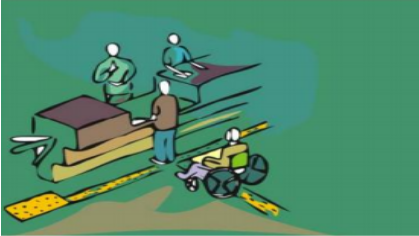
\includegraphics[width=.5\textwidth]{Fig/pupo.PNG}
{\footnotesize\center{\small Fonte: \cite{knuth:84}}} %citar e mudar fonte
\label{fig1}
\end{figure}

%\section{Figures and Captions}\label{sec:figs}

Utilize a expressão “Dados da pesquisa” ou “Elaborado pelos autores”, “Elaborado pelas autoras” caso sejam originais do manuscrito. Em caso de uso ou adaptação de material de outra fonte, indicá-la em forma de citação e colocar a referência completa na lista de referências ao final do manuscrito. Veja os exemplos.

\begin{quadro}[H]
\label{quad1}
\centering
\textbf{\caption{Total de documentos por programa de pós-graduação}}
\vspace{.3cm}
\begin{tabular}{|c|c|c|}
\cline{1-3}
 Autor & Título & Data \\ \cline{1-3}
 ABNT & NBR 6023 Referências  & 2018 \\ \cline{1-3}
 ABNT & NBR 6024 Numeração progressiva das seções de um documento & 2012 \\ \cline{1-3}
 ABNT & NBR 6028 Resumos & 2003 \\ \cline{1-3}
 ABNT & NBR 10520 Citações em documentos & 2002 \\ \cline{1-3}
 IBGE & Normas de apresentação tabular. 3. ed. & 1993 \\ \cline{1-3}
\end{tabular}
{\footnotesize\center{\small Fonte: \cite{knuth:84}}} %fonte
\end{quadro}

%\vspace{-1.5cm}
ATENÇÃO: Note que quadros contêm dados qualitativos e são fechados em todos os seus lados, enquanto tabelas contêm dados numéricos e devem ter as laterais abertas.
%\vspace{-1.5cm}

\begin{table}[H]
\label{tab1}
\centering
\caption{Avaliação de um periódico de Comunicação } 
\begin{tabular}{c|c|c|c|c|c|c}
\cline{1-7}
Critérios & Excelente & Bom & Regular & Ruim & Não conhece & Total\\ \cline{1-7}
Avaliação geral & 24\% & 32\% & 11\% & 6\% & 27\% & 100\%\\ \cline{1-7}
Qualidade artigos & 23\% & 28\% & 17\% & 5\% & 27\% & 100\% \\ \cline{1-7}
Contribuição para área & 31\% & 27\% & 7\% & 8\% & 27\% & 100\%\\ \cline{1-7}
Apresentação gráfica & 18\% & 28\% & 18\% & 9\% & 27\% & 100\% \\ \cline{1-7}
\end{tabular}
\vspace{0.3cm}
{\footnotesize\center{\small Fonte: \cite{knuth:84}}} %fonte
\end{table}

%COLCOCAR AS TABELAS



Exemplos de Gráficos
\begin{figure}[H]
\centering
\caption{Fonte: Elaborado pelos autores (2020)}
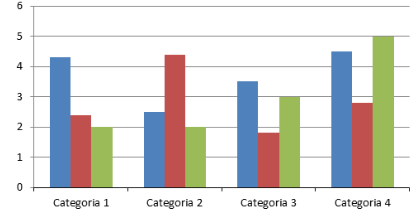
\includegraphics[width=15.0cm]{Fig/graf1.PNG}
{\footnotesize\center{\small Fonte: \cite{knuth:84}}} 
%Section~\ref{sec:figs}.
\label{graf1}
\end{figure}

\begin{figure}[H]
\centering
\caption{Gráfico 2 – Total de documentos por programa de pós-graduação } %Section~\ref{sec:figs}.
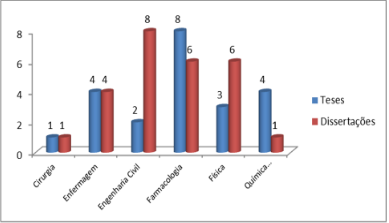
\includegraphics{Fig/grafico2.PNG}
{\footnotesize\center{\small Fonte: \cite{knuth:84}}}
\label{graf2}
\end{figure}


\section{CONCLUSÃO/CONSIDERAÇÕES FINAIS}
\label{Conclusão}

All images and illustrations should be in black-and-white, or gray tones,
excepting for the papers that will be electronically available (on CD-ROMs, internet, etc.). The image resolution on paper should be about 600 dpi for black-and-white images, and 150-300 dpi for grayscale images.  Do not include images with excessive resolution, as they may take hours to print, without any visible difference in the result. 

\section*{NOTAS EXPLICATIVAS \textcolor{red}{(opcional - se houver)}}
A numeração das notas explicativas é feita através de algarismos arábicos, devendo ser única e consecutiva, para cada artigo.

\section*{REFERÊNCIAS}
PUPO, D. T. Acessibilidade e inclusão: o que isto tem haver com os bibliotecários. In: PUPO, D.; MELO, A. M.; FERRES, S. F. Acessibilidade: discurso e prática nos cotidianos das bibliotecas. Campinas: Unicamp, 2008.

STUMPF, Ida Regina Chittó. Avaliação das revistas de Comunicação pela comunidade acadêmica da área. Em Questão, Porto Alegre, v. 9, n. 1, p. 25-38, jan./jun. 2003.

ASSOCIAÇÃO BRASILEIRA DE NORMAS TÉCNICAS (ABNT). NBR 6022: Informação e documentação - artigo em publicação periódica técnica e/ou científica – apresentação. Rio de Janeiro: ABNT, 2018b

ASSOCIAÇÃO BRASILEIRA DE NORMAS TÉCNICAS (ABNT). NBR 6023: informação e documentação - referências - elaboração. Rio de Janeiro: ABNT, 2018a.

ASSOCIAÇÃO BRASILEIRA DE NORMAS TÉCNICAS (ABNT). NBR 10520: informação e documentação – citações em documentos – apresentação. Rio de Janeiro: ABNT, 2002b.


\section*{APÊNDICE \textcolor{red}{(opcional)}}
O apêndice é um texto ou documento \textbf{elaborado} pelo autor do trabalho a fim de complementar o texto principal. Deve ser colocada em páginas distintas.

\section*{ANEXO \textcolor{red}{(opcional)}}
O anexo é um documento \textbf{não elaborado} pelo autor do trabalho. O intuito do anexo é de fundamentar, esclarecer, ilustrar e confirmar ideias abordadas no contexto do trabalho. Deve ser colocada em páginas distintas.


\section*{AGRADECIMENTOS \textcolor{red}{(opcional)}}
Este item destina-se a agradecer, sucintamente, pessoas, instituições, patrocinadores, que \textbf{realmente colaboraram} com o desenvolvimento do trabalho. Não diz respeito a agradecimentos pessoais. Deve ser colocada em páginas distintas.


\newpage

%\bibliographystyle{abnt}
\bibliography{bibliografia}

\end{document}
